\documentclass{article}
\usepackage[utf8]{inputenc}
\usepackage{tabu}
\usepackage{pgf}
\usepackage{tikz}
\usetikzlibrary{arrows,automata}
\begin{document}
\textbf{Mechanism}: There are five compartments in the model. The compartments are normal susceptible population, enthusiastic susceptible population, exposed population, infected population and skeptic population. The normal susceptible population represents the number of twitter accounts of people who have not seen the particular story on twitter and are neutral about the topic related to it. On the contrary, the enthusiastic susceptible population is the number of twitter accounts of people who have not seen the story on twitter but care deeply about the topic related to it. The exposed population is the number of twitter accounts of people have been exposed to the story and have not reacted to it yet. The infected population is the number of twitter accounts of people that have reacted to the story on twitter. The skeptic population represents the number of twitter accounts of people who have been exposed to the story but will not react to it on twitter. 
\\The presence of the infected population acts as recruitment of the susceptible populations to itself. If there is contact between infected and susceptible, with some probability people from the susceptible population will react to the story and move to the infected population. The rest of the contacted people will move to the exposed population. Note that this applies to both susceptible populations. Similarly, the presence of the skeptic population acts as recruitment. If there is contact between skeptic and susceptible, with probability some people from the susceptible population will move to the skeptic population. The rest of the contacted people will move to the exposed population. The model assumes that the presence of the skeptic population has no effect on the enthusiastic susceptible population. From the exposed population, people can move to the infected population with the help of further contact with the infected population or on their own. The model assumes that the enthusiastic population is much more likely to react to the story than the normal population. 
\begin{center}
    

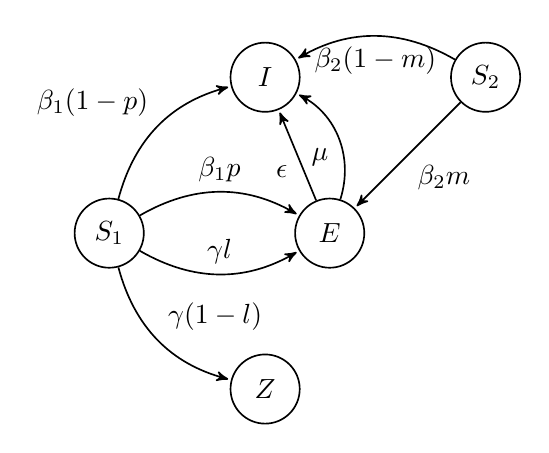
\begin{tikzpicture}[->,>=stealth',shorten >=1pt,auto,node distance=2.8cm,
                    semithick]
  \node[state] (S1)                    {$S_1$};
  \node[state]              (I)[above right of=S1] {$I$};
  \node[state]              (Z)[below right of=S1] {$Z$};
  \node[state]              (E)[right of=S1] {$E$};
  \node[state]              (S2)[right of=I] {$S_2$};

  \path (S1) edge   [bend left]                 node{${\beta}_1(1-p)$} (I);
  \path (S1) edge   [bend left]                 node{${\beta}_1 p$} (E);
  \path (S1) edge   [bend right]                 node{${\gamma}l$} (E);
  \path (S1) edge   [bend right]                 node{${\gamma}(1-l)$} (Z);
  \path (S2) edge   [bend right]                node{${\beta}_2(1-m)$} (I);
  \path (S2) edge                   node{${\beta}_2 m$} (E);
  \path (E) edge    [bend right=40]               node{$\mu$} (I);
  \path (E) edge                  node{$\epsilon$} (I);
\end{tikzpicture}
\end{center}
\begin{center}

\begin{tabu} to 0.8\textwidth { | X[l] | X[r] |}
 \hline
 Parameters and variables& Explanation \\
 \hline
 $S_1$  & Normal susceptible population  \\
\hline
 $S_2$ & Enthusiastic susceptible population\\
 \hline
 $E$ & Exposed population  \\
 \hline
 $I$ & Infected population  \\
 \hline
 $Z$ & Skeptic population \\
  \hline
 $\gamma$ & $S_1-Z$ contact rate \\
 \hline
 ${\beta}_1$ & $S_1-I$ contact rate \\
 \hline
 ${\beta}_2$ & $S_2-I$ contact rate \\
 \hline
 $\mu$ & $E-I$ contact rate \\
 \hline
 $p$ & $S_1-E$ conversion $\mathbf{P}$ given contact with infected \\
 \hline
 $1-p$ & $S_1-I$ conversion $\mathbf{P}$ given contact with infected \\
 \hline
 $l$ & $S_1-E$ conversion $\mathbf{P}$ given contact with skeptic \\
 \hline
 $1-l$ & $S_1-Z$ conversion $\mathbf{P}$ given contact with skeptic \\
 \hline
 $m$ & $S_2-E$ conversion $\mathbf{P}$ given contact with infected \\
 \hline
 $1-m$ & $S_2-I$ conversion $\mathbf{P}$ given contact with infected \\
 \hline
 $\epsilon$ & incubation rate \\
 \hline
 

\end{tabu}
\end{center}
\textbf{Constraints}: 
$${\beta}_1 < {\beta}_2$$  
$$0\leq m<p\leq 1$$  
$$0\leq l \leq 1$$ 
$$N = S_1 + S_2 + E + Z + I$$
$$\frac{dN}{dt}=0$$
\\
\textbf{Equations}: 
$$ \frac{dS_1}{dt} = -{\beta}_1 S_1\frac{I}{N} -\gamma S_1\frac{Z}{N}$$
$$ \frac{dS_2}{dt} = -{\beta}_2 S_2\frac{I}{N}$$
$$\frac{dI}{dt} = {\beta}_1 (1-p)S_1\frac{I}{N} + {\beta}_2 (1-m)S_2\frac{I}{N} + \epsilon E + \mu E\frac{I}{N}$$
$$\frac{dE}{dt} = {\beta}_1 pS_1\frac{I}{N} + {\beta}_2 mS_2\frac{I}{N} + \gamma       lS_1\frac{Z}{N} - \mu E\frac{I}{N} - \epsilon E$$
$$\frac{dZ}{dt} =  \gamma (1-l)S_1\frac{Z}{N}$$
\end{document}
